\section{ Two body elliptical orbits: Two body H. velocity and acceleration  }\label{sec:q2}    
This entire question is sourced from chapters 2.3, 5.1, 6.2 and 7.1.
\subsection{a. Circular velocity and escape velocity as function of r}
Starting with
\begin{equation}
e^2 = 1 - \frac{r V^2}{\mu}\Bigg(2 - \frac{r V^2}{\mu}\Bigg) \cos^2 \gamma
\label{start}
\end{equation}
The following trigonometric identity is used:
\begin{equation}
\sin^2\gamma + \cos^2\gamma = 1
\end{equation}
\begin{equation}
e^2 = \cos^2\gamma + \sin^2\gamma - \frac{r V^2}{\mu}\Bigg(2 - \frac{r V^2}{\mu}\Bigg) \cos^2 \gamma
\end{equation}
\begin{equation}
e^2 = \sin^2\gamma + \cos^2\gamma \Bigg[1-\frac{2rV^2}{\mu}+\Big(\frac{rV^2}{\mu}\Big)^2 \Bigg]
\end{equation}
Rewriting to

\begin{equation}
e^2 = \sin^2\gamma + \cos^2\gamma \Bigg[\Big(1-\frac{rV^2}{\mu}\Big)\Big(1-\frac{rV^2}{\mu}\Big)\Bigg]^2
\end{equation}

\begin{equation}
e^2 = \sin^2\gamma + \cos^2\gamma\Bigg[1-\frac{rV^2}{\mu}\Bigg]^2
\end{equation}
For circular orbit, plugging in e=0 yields:

\begin{equation}
\sin^2\gamma = -\cos^2\gamma\Bigg[1-\frac{rV^2}{\mu}\Bigg]^2
\end{equation}

\begin{equation}
\frac{\sin^2\gamma}{\cos^2\gamma} = - \Bigg[1-\frac{rV^2}{\mu}\Bigg]^2
\end{equation}
\begin{equation}
\tan^2\gamma = - \Bigg[1-\frac{rV^2}{\mu}\Bigg]^2
\end{equation}
\begin{equation}
\gamma = \arctan\Bigg(\sqrt{-\Big[1-\frac{rV^2}{\mu}\Big]^2}\Bigg)
\end{equation}
For real solutions, the following condition applies:
\begin{equation}
\frac{rV^2}{\mu} = 1
\end{equation}
Where V is the circular velocity V\textsubscript c. Rewriting yields:
\begin{equation}
V_c = \sqrt[]{\frac{\mu}{r}}
\end{equation}
Next, realizing that for escape velocity, e = 1, this value is plugged into the expression from eq.\ref{start}.
\begin{equation}
e^2 = 1 = 1 - \frac{r V^2}{\mu}\Bigg(2 - \frac{r V^2}{\mu}\Bigg) \cos^2 \gamma
\end{equation}
\begin{equation}
\frac{r V^2}{\mu}\Bigg(2 - \frac{r V^2}{\mu}\Bigg) \cos^2 \gamma = 0
\end{equation}
The two solutions to this equation are:
\begin{equation}
\frac{r V^2}{\mu}\cos^2 \gamma = 0 \lor \Bigg(2-\frac{rV^2}{\mu}\Bigg) = 0
\end{equation}
The first solution is considered:
\begin{equation}
\frac{r V^2}{\mu}\cos^2 \gamma = 0
\end{equation}
Where, assuming neither \textit{r} nor \textit{V} are equal to zero, the path angle is required to be equal to 90 degrees. The physical meaning would be that the body would rectilinearly move away from the centre of attraction, which bears no physical meaning and therefore this solution is a trivial one.
Now, the second solution is considered:
\begin{equation}
\Bigg(2-\frac{rV^2}{\mu}\Bigg) = 0
\end{equation}
Rewriting yields:
\begin{equation}
V = \sqrt{\frac{2\mu}{r}}
\end{equation}
And since
\begin{equation}
V_c = \sqrt{\frac{\mu}{r}}
\end{equation}
And therefore
\begin{equation}
V_{esc} = \sqrt{2} V_c
\end{equation}
\subsection{b. Derivation of the expression for the semi-major axis for an elliptical orbit}
The following expression is to be derived:
\begin{equation}
a = \frac{\mu/2}{\mu/r - V^2/2}
\end{equation}
Starting with the given equations
\begin{equation}
p = \frac{H^2}{\mu}
\end{equation}
and
\begin{equation}
H = r V \cos\gamma
\end{equation}
Substitution yields
\begin{equation}
p = \frac{r^2V^2\cos^2\gamma}{\mu}
\label{p}
\end{equation}
Now considering the orbital equation
\begin{equation}
r = \frac{p}{1+e\cos\theta}
\label{r}
\end{equation}
Considering eq. \ref{r} at respectively 0 and 180 degrees for perigee and apogee:
\begin{equation}
2a = r_a + r_p = \frac{p}{1+e\cos0} + \frac{p}{1+e\cos180} = \frac{p}{1-e} + \frac{p}{1+e} = \frac{2p}{1-e^2}
\end{equation}
Therefore
\begin{equation}
a = \frac{p}{1-e^2}
\label{aeq}
\end{equation}
Now for the big finale, substitution of eq. \ref{start}, \ref{p} and \ref{aeq} yields:
\begin{equation}
a = \frac{r^2 V^2 \cos^2 \gamma}{\mu \Bigg[ 1 - \Big(1 - \frac{r V^2}{\mu}\Big[2 - \frac{r V^2}{\mu}\Big]\cos^2\gamma \Big) \Bigg]}
\end{equation}
\begin{equation}
a = \frac{r^2 V^2 \cos^2 \gamma}{r V^2 \cos^2 \gamma \Big[2 - \frac{r V^2}{\mu} \Big]} 
\end{equation}
\begin{equation}
a = \frac{r}{2 - \frac{r V^2}{\mu}} = \frac{r}{r\Big[ \frac{2}{r}-\frac{V^2}{\mu}\Big]} = \frac{\mu}{\mu} \frac{1}{\frac{2}{r} - \frac{V^2}{\mu}}
\end{equation}
\begin{equation}
a = \frac{\mu}{\frac{2\mu}{r} - V^2} = \frac{1/2}{1/2} \frac{\mu}{\frac{2\mu}{r} - V^2} = \frac{\mu/2}{\mu/r - V^2/2}
\end{equation}
Q.E.D.
\subsection{c. Proof of constant energy sum}
Considering the conservation of energy
\begin{equation}
E_k + E_p = C
\end{equation}
Where
\begin{equation}
E_k = \frac{1}{2}mV^2
\end{equation}
and
\begin{equation}
E_p = -m\frac{\mu}{r}
\end{equation}
And because m is constant for a body
\begin{equation}
\frac{1}{2} V^2 - \frac{\mu}{r} = C
\label{constant1}
\end{equation}
Considering the equation for the semi-major axis from subquestion (b), it is observed that a and mu always have a positive and nonzero value. Thus it can be stated that 
\begin{equation}
\frac{\mu}{r} - \frac{1}{2}V^2 > 0 
\end{equation}
or
\begin{equation}
\frac{1}{2} V^2 - \frac{\mu}{r} < 0
\label{constant2}
\end{equation}
Comparing equations \ref{constant1} and \ref{constant2}, the definition is proven, the proof holds for orbits with an eccentricity between 0 and 1 due to the definition of the semi-major axis.
\subsection{d. Velocity at pericenter and apocenter}
Considering
\begin{equation}
V^2 = \mu \Big(\frac{2}{r}-\frac{1}{a}\Big)
\label{start}
\end{equation}
For the pericenter it is known that
\begin{equation}
r_p = \frac{p}{1+e}
\end{equation}
Substituting
\begin{equation}
p = a (1-e^2)
\end{equation}
yields
\begin{equation}
r_p = \frac{a(1-e^2)}{1+e}=a(1-e)
\end{equation}
Substituting this in eq. \ref{start} results in
\begin{equation}
V_p = \sqrt{\mu \Big( \frac{2}{a(1-e)}-\frac{1}{a} \Big)} = \sqrt{\frac{2\mu}{a(1-e)} - \frac{\mu(1-e)}{a(1-e)}}
\end{equation}
So
\begin{equation}
V_p = \sqrt{\frac{2\mu - \mu + e\mu}{a(1-e)}} = \sqrt{\frac{\mu(1+e)}{a(1-e)}} = \sqrt{\frac{\mu}{a(1-e)}(1+e)}
\label{perigee1}
\end{equation}
Consider the circular velocity at perigee 
\begin{equation}
V_{cp} = \sqrt{\frac{\mu}{r_p}} = \sqrt{\frac{\mu}{a(1-e)}}
\end{equation}
\begin{equation}
V_{cp}^2 = \frac{\mu}{a(1-e)}
\label{perigee2}
\end{equation}
Substitution of eq. \ref{perigee2} into eq. \ref{perigee1} yields:
\begin{equation}
V_p = \sqrt{V_{cp}^2(1+e)} = V_{cp} \sqrt{1+e}
\end{equation}
This is now written as
\begin{equation}
V_p^2 = V_{cp}^2 (1+e)
\end{equation}

\bigskip

And now for apocenter
\begin{equation}
r_a = \frac{p}{1-e} = \frac{a(1-e^2)}{1-e}=\frac{a(1+e)(1-e)}{(1-e)} = a(1+e)
\end{equation}
Substituting this into eq. (2) as given in the exam, yields

\begin{equation}
V_a^2=\mu \Big(\frac{2}{r_a}-\frac{1}{a}\Big) = \mu \Big(\frac{2}{a(1+e)}-\frac{1(1+e)}{a(1+e)}\Big)
\end{equation}
\begin{equation}
=\mu \Big(\frac{1-e}{a(1+e)}\Big) = \frac{\mu}{a(1+e)}(1-e)
\end{equation}
Circular velocity at apogee is
\begin{equation}
V_{ca} = \sqrt{\frac{\mu}{r_a}} = \sqrt{\frac{\mu}{a(1+e)}}
\end{equation}
\begin{equation}
V_{ca}^2 = \frac{\mu}{a(1+e)}
\end{equation}
Substituting in the same way as demonstrated for the perigee velocity:
\begin{equation}
V_a^2 = V_{ca}^2(1+e)
\end{equation}
\subsection{e. Ratio between maximum/minimum velocity in an elliptical orbit}
\begin{equation}
\frac{V_{max}}{V_{min}} = \frac{1+e}{1-e}
\end{equation}
Knowing that the highest velocity is at the pericenter and the lowest velocity at the apocenter, it is stated that:
\begin{equation}
V_{max} = V_p = V_{cp} \sqrt{1+e} = \sqrt{\frac{\mu(1+e)}{a(1-e)}}
\end{equation}
\begin{equation}
V_{min} = V_a = V_{ca} \sqrt{1-e} = \sqrt{\frac{\mu(1-e)}{a(1+e)}}
\end{equation}
Therefore
\begin{equation}
\frac{V_{max}}{V_{min}} = \frac{\sqrt{\frac{\mu(1+e)}{a(1-e)}}}{\sqrt{\frac{\mu(1-e)}{a(1+e)}}} =\sqrt{ \frac{\frac{\mu}{a}}{\frac{\mu}{a}}} \sqrt{\frac{\frac{1+e}{1-e}}{\frac{1-e}{1+e}}} = \sqrt{\frac{1+e}{1-e} \frac{\frac{1}{1-e}}{\frac{1}{1+e}}} = \sqrt{\frac{(1+e)^2}{(1-e)^2}} = \frac{1+e}{1-e}
\end{equation}
\clearpage
\subsection{f. Semi-major axis for hyperbolic trajectory}
First, a sketch of a hyperbolic trajectory: 
\begin{figure}[h]
\centering
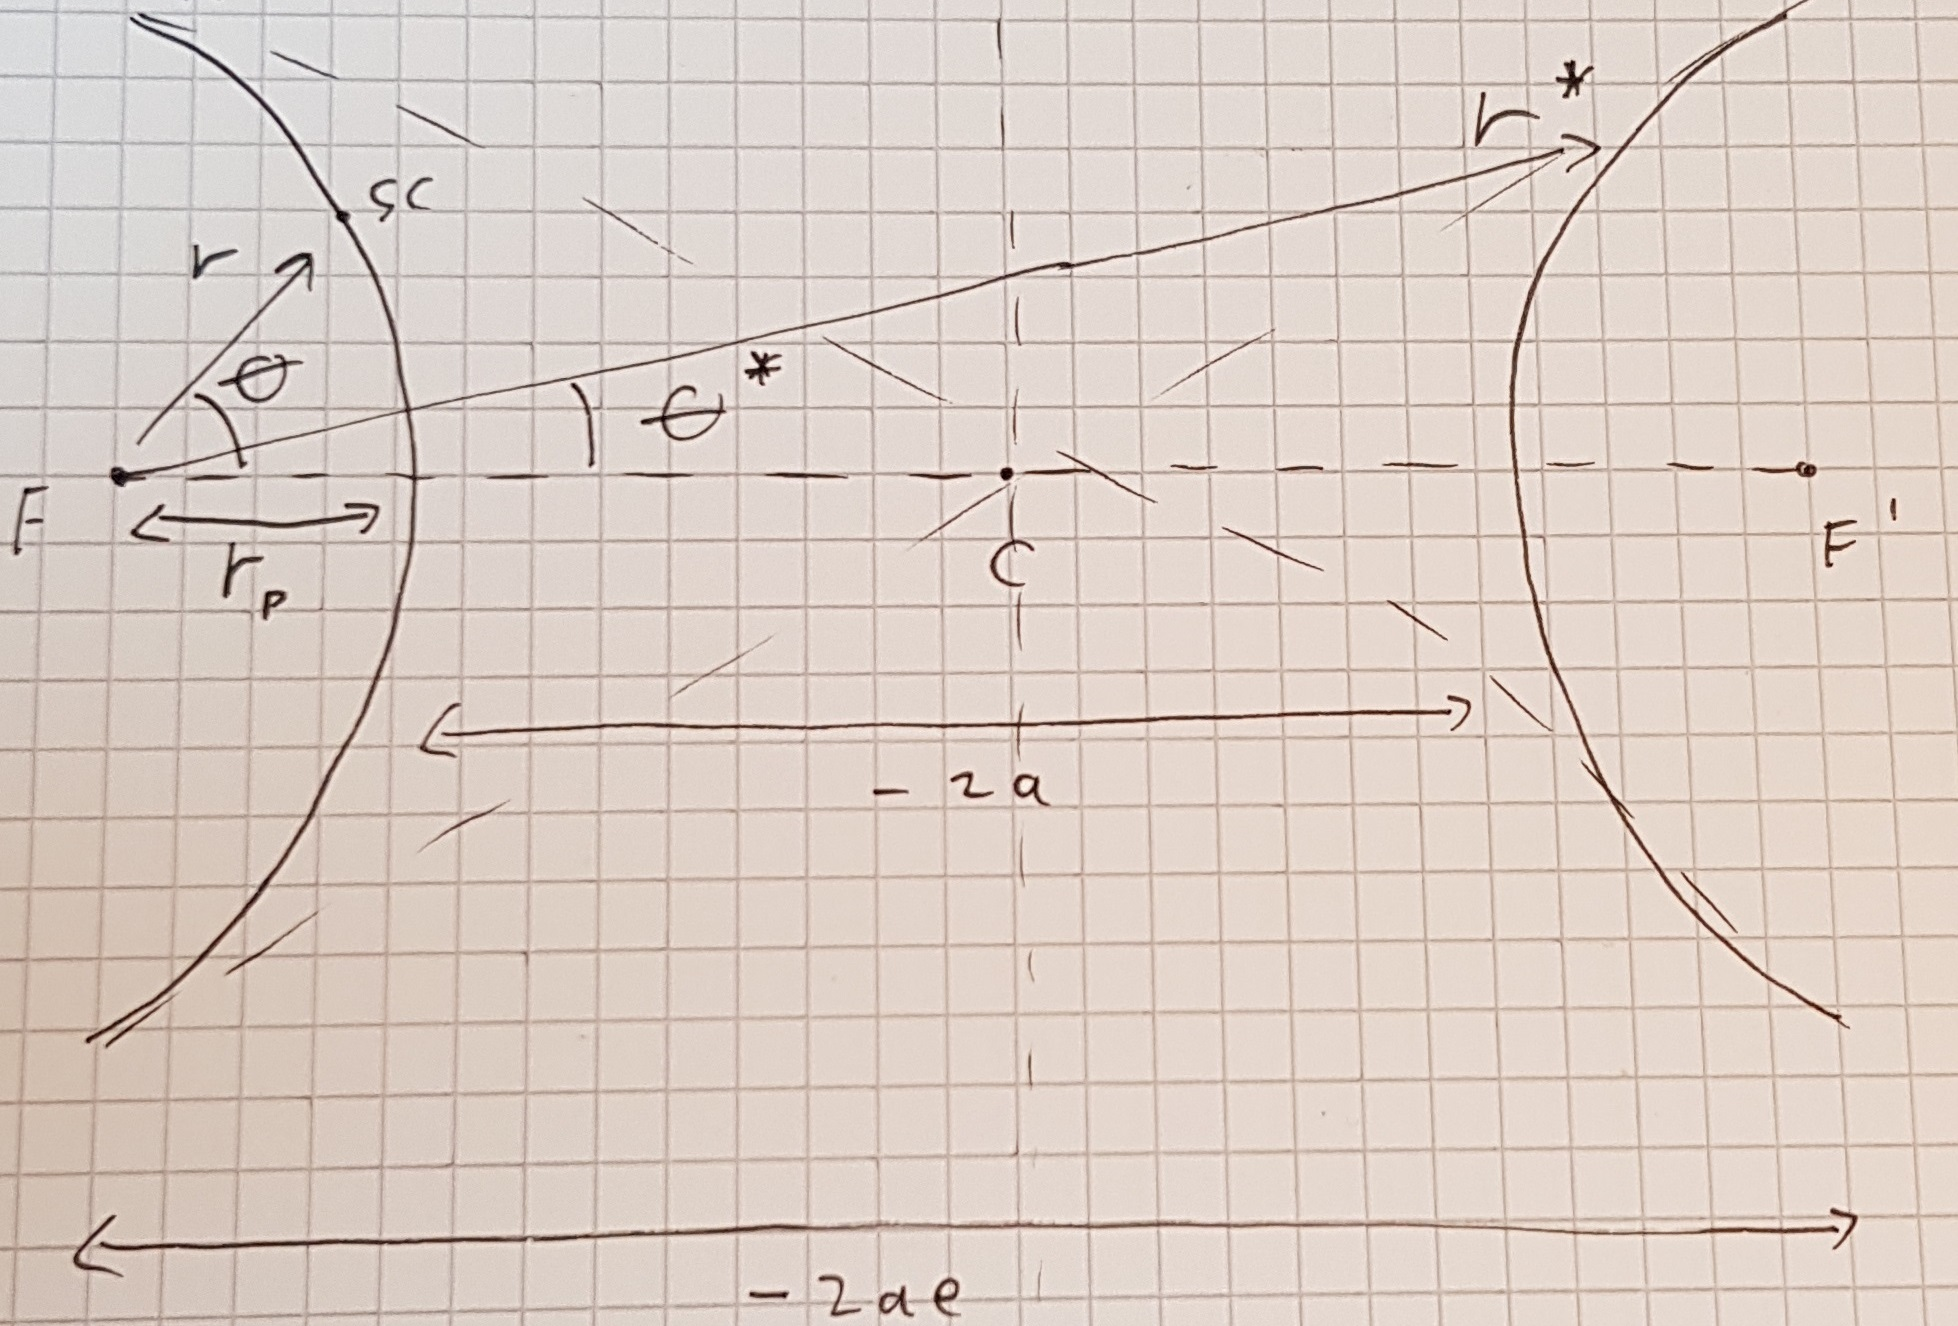
\includegraphics[scale=0.15]{chapters/sketch1.jpg}
\caption{Sketch, Artemis2020, 2019}
\end{figure}

For a hyperbolic trajectory, 
\begin{equation}
e>1
\end{equation}
holds.
At 
\begin{equation}
\theta_p = 0
\end{equation}
So
\begin{equation}
r_p = \frac{p}{1+e\cos 0} = \frac{p}{1+e} = a(1-e)
\end{equation}
Distance CF from center to focal point for elliptical orbits:
\begin{equation}
FC = r_p - a = a(1-e) - a = - ae
\end{equation}
For a hyperbolic orbit it holds that (see sketch)
\begin{equation}
- 2 ae = 2 r_p - 2 a
\end{equation}
\begin{equation}
2a - 2ae = 2a(1-e) = 2r_p
\end{equation}
Thus
\begin{equation}
a = \frac{r_p}{1-e}
\end{equation}
For this type of trajectory, a negative semi-major axis is assumed. This is the shortest distance between both curves shown, expressed as:
\begin{equation}
-2a = r^*(\theta^* = 0) - r(\theta = 0)
\end{equation}
Calculating r*
\begin{equation}
r^* = \frac{-p}{1-e\cos 0} = \frac{-p}{1-e}
\end{equation}
Calculating r
\begin{equation}
r = \frac{p}{1+e\cos 0} = \frac{p}{1+e}
\end{equation}
Combining these three equations yields
\begin{equation}
-2a = \frac{-p}{1-e} - \frac{p}{1+e} = \frac{-p(1+e) - p(1-e)}{(1-e)(1+e)} = \frac{-p -pe -p +pe}{1-e^2} = \frac{-2p}{1-e^2}
\end{equation}
Therefore
\begin{equation}
2a = \frac{2p}{1-e^2}
\end{equation}
And thus
\begin{equation}
a = \frac{p}{1-e^2}
\end{equation}
Q.E.D.
\clearpage
\subsection{g. Local velocity in hyperbolic orbit}
It is asked to prove the following equation
\begin{equation}
V^2 = V_{esc}^2+V_{\infty}^2
\end{equation}
First, consider the vis-vica equation
\begin{equation}
V^2 = \mu \Big[\frac{2}{r} - \frac{1}{a}\Big]
\end{equation}
At infinity, the first term inside the square brackets approaches zero. Therefore:
\begin{equation}
V_{\infty}^2 = -\frac{\mu}{a}
\end{equation}
Consider now the definition of the escape velocity
\begin{equation}
V_{esc} = \sqrt{2} V_c = \sqrt{\frac{2\mu}{r}}
\end{equation}
Hence
\begin{equation}
V_{esc}^2 = \frac{2\mu}{r}
\end{equation}
Plugging these equations into the vis-viva equation:
\begin{equation}
V^2 = \frac{2\mu}{r} - \frac{\mu}{r} = V_{\infty}^2-V_{esc}^2
\end{equation}
\subsection{h. Ratio between maximum and minimum velocity in hyperbolic orbit}
Prove that:
\begin{equation}
\frac{V_{max}}{V_{min}} = \sqrt{\frac{e+1}{e-1}}
\end{equation}
Realizing once again that maximum velocity occurs at the pericenter,
\begin{equation}
V_{max}^2 = V_p^2 = V_{cp}^2(1+e) = \sqrt{\frac{\mu(1+e)}{a(1-e)}}
\end{equation}
Realizing that minimum velocity occurs at the apocenter, which for a hyperbolic orbit is at infinity,
\begin{equation}
V_{min} = V_{\infty} = \sqrt{-\frac{\mu}{a}}
\end{equation}
Combining yields:
\begin{equation}
\frac{V_{max}}{V_{min}} =\frac{\sqrt{\frac{\mu(1+e)}{a(1-e)}}}{\sqrt{-\frac{\mu}{a}}}
 = \frac{\sqrt{\frac{\mu}{a}}}{\sqrt{\frac{\mu}{a}}} \frac{-\sqrt{1+e}}{1-e} = \sqrt{\frac{e+1}{e-1}}
\end{equation}
Q.E.D.
\clearpage









